\chapter{Methodology}

Procedure of getting data to perform an analysis
from the collected data is very important. In order 
to get a precise Earth's limb $\gamma$-ray spectrum to
trace back the incident proton spectrum, it is crucial 
to carefully determine the selection criteria from raw 
data in many angle base on the objectives. This chapter 
will begin by giving information of $\gamma$-ray flux extraction 
by providing information of data filtering and 
the extracting process from scratch. Secondly, hadronic collision 
model that forwardly yield the $\gamma$-ray spectrum 
will be discuss and tracing the incident CR's proton 
spectrum algorithm from heuristic optimization. Lastly,
the last sub-chapter contains details of statistical analysis.

\begin{figure}[h!]
    \centering
    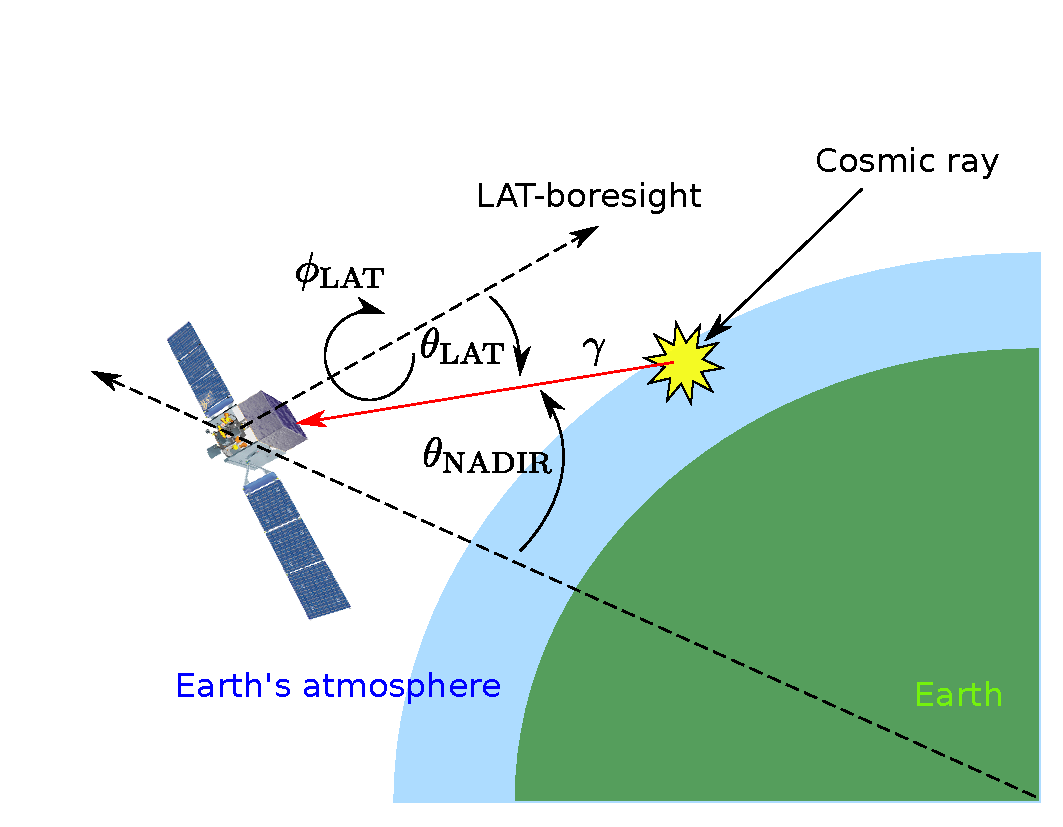
\includegraphics[width=0.7\textwidth]{content/methodology/figures/gamma_production_schematic}
    \caption{Schematics of $\gamma$-ray production}
    \label{fig:gamma_emis_sp}
\end{figure}

The required fundamental concept of spacecraft orientation and 
the observations of Earth's limb $\gamma$ emission is another crucial
concept. The Figure \ref{fig:gamma_emis_sp} demonstrates the important
axis which are $\theta_\text{NADIR}$ represent the angle of how further
from Earth's center in the spacecraft point of view as well as 
$\theta_\text{LAT}$ to the angle from incident $\gamma$-ray to the 
detector normal in domain between 0 to 90\textdegree
and $\phi_\text{LAT}$ as the clockwise angle from 0 to 2$\pi$.


\section{Data selection}
In this work, 9 years of LAT's flight data has been used
to analyze reconstructed photon and their metadata of spacecraft
log recorded in a similar format periodically every half minutes.
The reconstructed algorithm version is the latest version which is
Pass 8 with the cleanest photon events that exists from \textit{Fermi}-LAT
data catalogues called ULTRACLEANVETO. To be more precise, the photon 
data is collected from publically available raw FITs file from the 

Only high energy limb's photon will be selected from 10 GeV up to 1 TeV.
It makes the tracebacking analysis for gaining the information of
CR proton spectrum in rigidity between 60 GV to 2 TV. The definition 
of $\gamma$-ray's limb regiom is obtained from \cite{FermiEarth09} in 
a given nadir angle from 68.4\textdegree to 70.0\textdegree. 
The maximum of incident angle ($\theta_\text{LAT}$) that was
measured from the z-axis of the LAT's foresight is 70\textdegree.


\section{Flux extraction}

There are multiple step from trivial to complex calculation to 
obtain the differential flux. The definition when saying flux 
is actually a differential flux that be calculated one
chunk of energy range at a time as Equation \ref{eq:def_flux}

\begin{equation}
    \textbf{Flux} \equiv \frac{dN_\gamma}{dE} = \frac{\int_\text{Limb region}(\text{Count map}/\text{Exposure map})}{\Delta\Omega\Delta E}.
    \label{eq:def_flux}
\end{equation}
Since the CR spectrum follows a power law as the exponential form 
 $dN/dR \propto R^\gamma$ as mentioned in the background section.
Then the log-log relation of the flux versus rigidity would behave 
like a trivial linear trend in the plot. Not only the rigidity, but 
in the high energy CR like 10 GeV also makes the energy of the particle
almsot the same as the rigidity does. Consequently, the $\gamma$-ray
spectrum is equally divived in the energy space in the log scale for 
50 bins.

To get the spectrum, it is obvious to construct the histogram 
with 50 bins in a given energy scale as explained in the previous paragraph.
The flux of each bin could be computed separately by initializing 
the empty count map and the exposure map where it represents the
exposure time and the effectiveness of the spacecraft when looking 
at each angle in the sky. Let regards the following example for 
a deeper understanding. The ideal scenario is when incident $\gamma$-ray
walk pass through the LAT in a normal line of the detector. 
Definitely, the performance would be the highest as it could do.
On the other hand, if the incident $\gamma$-ray arrive with high 
tile angle from the LAT's plane (High $\theta_\text{LAT}$).
An angle resolution is selected to be 2\textdegree in $\phi_\text{NADIR}$
and 0.1\textdegree in $\theta_\text{NADIR}$. The reason behind these 
number is simply from the toy experiment of plotting the result 
in the 2D histogram and it is selected to be the one as the bin value 
is not too noist. In another words, it should not be too small so that 
the result is not too noisy and it is should not so big due to the 
limb region could not be seen clearly which leads to the matched photon 
mixed up with the Earth's $\gamma$-rays and collecting too many primary 
CR photon.


Basically, the procedure is summarized in these following steps.
\begin{enumerate}
    \item Make 2D histograms with 25 bins per decade of energy
    \item Select photon data and fill in the 2D histograms
    \item Calculate exposure maps which include the effective area
    and livetime of the LAT as it observed the Earth    
    \item Compute the flux by applying Equation \ref{eq:def_flux} in for bin 
    \item Taking consider background subtraction from a average
    uniform background photon distribution by treating bin by bin 
\end{enumerate}


\subsection{Exposure map gathering}
In fact, step 3 is the most complicate stage in this work.
Practically, $Fermi$-LAT was designed for observing the space which
makes the spacecraft logging in equatorial coordinates not for the 
Earth's polar coordinates. The LAT position is recorded in 
equatorial coordinates as well as the LAT's boresight of the detector
plane to log their orientation during the orbit. In the end of the day,
the coordinates transformation would be perform from multiple frame 
of references to LAT boresight for acquiring the exposure of LAT's FoV
and reference the effectiveness from LAT's boresight angle dependency.
The following content is the full detail of how things going on 
under the hood.

\subsubsection{Coordinate Transformations}

Firstly, the spacecraft orbit is recorded in the equatorial coordinate
which in spherical point of view. Defining the cartesian coordinate
that share the origin between celestial point of view and the spacecraft 
by letting one axis point to the spacecraft could assist the calculation
more convenient as the Figure \ref{fig:coord_eq_sp}. Please note that 
the x-axis in equatorial coordinate is called ``Equinox''.

\begin{figure}[h!]
    \centering
    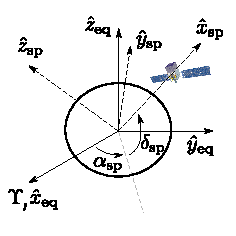
\includegraphics[width=0.5\textwidth]{content/methodology/figures/coord_eq_sp.pdf}
    \caption{Coordinate transform between celestial and spacecraft}
    \label{fig:coord_eq_sp}
\end{figure}


However, mapping into the cartesian 
coordinate by adopting a unit vector in 3 dimensions has been written
as Equation \ref{eq:tf_eq_sp} and the synbolic transformation is 
represented in Equation \ref{eq:rep_tf_eq_sp}.

\begin{equation}
    \begin{split}
    \hat{x}_\text{sp} &= \cos\delta_\text{sp}\cos\alpha_\text{sp}\hat{x}_\text{eq} + \cos\delta_\text{sp}\sin\alpha_\text{sp}\hat{y}_\text{eq} + \sin\delta_\text{sp}\hat{z}_\text{eq}\\
    \hat{z}_\text{sp} &= - \sin\delta_\text{sp}\cos\alpha_\text{sp}\hat{x}_\text{eq} + \sin\delta_\text{sp}\sin\alpha_\text{sp}\hat{y}_\text{eq} + \cos\delta_\text{sp}\hat{z}_\text{eq} \\
    \hat{y}_\text{sp} &= \hat{z}_\text{sp} \times \hat{x}_\text{sp}
    \end{split}
    \label{eq:tf_eq_sp}
\end{equation}

\begin{equation}
    \hat{r}_\text{sp} \equiv T_{\text{eq}\rightarrow\text{sp}} (\delta_\text{sp}, \alpha_\text{sp}) \hat{r}_\text{eq}
    \label{eq:rep_tf_eq_sp}
\end{equation}

The transformation matrix $T_{\text{eq}\rightarrow\text{sp}}$ has been implemented as a matrix in practical
analysis due to the convenient for calculation and the compaction 
in the programming point of view.

Secondly, LAT's boresight coordinates is also referenced in equatorial 
coordinates. Figure \ref{fig:coord_eq_p} demonstrates the relation between
an incident plane of detector on equatorial coordinate and the 
nadir angle for regarding the exposure from LAT to Earth.

\begin{figure}[h!]
    \centering
    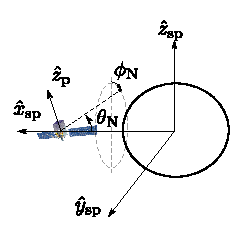
\includegraphics[width=0.5\textwidth]{content/methodology/figures/coord_eq_p.pdf}
    \caption{Coordinate transform between spacecraft and nadir angle}
    \label{fig:coord_eq_p}
\end{figure}

Unquestionably, it have to be converted into a cartesian 
point of view to do a mathemetical operation for simplicity. A 
full representation of the coordinates could be written as Equation \ref{eq:tf_eq_p}
and the compact form is in the Equation \ref{eq:rep_tf_eq_p}.

\begin{equation}
    \begin{split}
    \hat{x}_\text{p} &= \cos\delta^\text{x}_\text{p}\cos\alpha^\text{x}_\text{p}\hat{x}_\text{eq} + \cos\delta^\text{x}_\text{p}\sin\alpha^\text{x}_\text{p}\hat{y}_\text{eq} + \sin\delta^\text{x}_\text{sp}\hat{z}_\text{eq}\\
    \hat{z}_\text{p} &= \cos\delta^\text{z}_\text{p}\cos\alpha^\text{z}_\text{p}\hat{x}_\text{eq} + \cos\delta^\text{z}_\text{p}\sin\alpha^\text{z}_\text{p}\hat{y}_\text{eq} + \sin\delta^\text{z}_\text{sp}\hat{z}_\text{eq}\\
    \hat{y}_\text{p} &= \hat{z}_\text{p} \times \hat{x}_\text{p}
    \end{split}
    \label{eq:tf_eq_p}
\end{equation}

\begin{equation}
    \hat{r}_\text{p} \equiv T_{\text{eq}\rightarrow\text{p}} (\delta^\text{x}_\text{p}, \alpha^\text{x}_\text{p}, \delta^\text{z}_\text{p}, \alpha^\text{z}_\text{p}) \hat{r}_\text{eq}
    \label{eq:rep_tf_eq_p}
\end{equation}

Similarly, $T_{\text{eq}\rightarrow\text{p}}$ is also considered as 
a transformation matrix in the computation for monotizing the source 
code as well as keeping consistency in the logic.

Again, all those representation just for mapping the LAT's boresight
coordinate to link with the nadir coordinate to accumulate the 
exposure from the spacecraft's FoV. The spacecraft coordinate can be 
written as an dependency of Earth's poalr coordinate as Equation \ref{eq:def_r0}
in the cartesian system.

\begin{equation}
    \hat{r}^\text{o}_\text{sp} (\theta_\text{N}, \phi_\text{N}) \equiv -\cos\theta_\text{N}\hat{x}_\text{sp} + \sin\theta_\text{N}\cos\phi_\text{N}\hat{z}_\text{sp} + \sin\theta_\text{N}\sin\phi_\text{N}\hat{y}_\text{sp}
    \label{eq:def_r0}
\end{equation}

By the end of the day, extracting the relations to simplify the 
LAT's boresight coordinate could be contained by one inversion of 
transformation matrix from equatorial to spacecraft and transform it 
to plane of detector as written in the compact form in the Equation 
\ref{eq:def_r0_to_rp}.

\begin{equation}
    \hat{r}^\text{o}_\text{p} (\theta_\text{N}, \phi_\text{N}) = T_{\text{eq}\rightarrow\text{p}} (\delta^\text{x}_\text{p}, \alpha^\text{x}_\text{p}, \delta^\text{z}_\text{p}, \alpha^\text{z}_\text{p}) \left[T_{\text{eq}\rightarrow\text{sp}} (\delta_\text{sp}, \alpha_\text{sp})\right]^{-1} \hat{r}^\text{o}_\text{sp} (\theta_\text{N}, \phi_\text{N})
    \label{eq:def_r0_to_rp}
\end{equation}

\begin{figure}[h!]
    \centering
    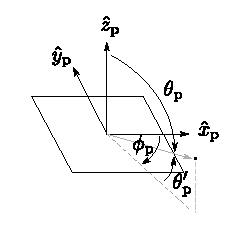
\includegraphics[width=0.5\textwidth]{content/methodology/figures/coord_plane}
    \caption{Detector's boresight in cartesian and polar coordinate}
    \label{fig:tf_lat_pol_car}
\end{figure}

Geometrically, angular coordinate of LAT plane could be obtained from
normalized component of the cartesian unit vector as in Figure
\ref{fig:tf_lat_pol_car}. The exposure accumulation has been
calculated in every single grid from the previous relation.

\subsubsection{Parallel Computations}

From the previous section, it is obvious that the complexity of 
the code becoming large due to the transformation operation.
For example, a plain matrix inversion cost $\mathcal{O}(n^3)$ where 
n is 3 because it is 3 by 3 matrix in this case. Not only the inversion,
but the matrix multiplication also cost the same amount of
complexity which cause a long run in the execution time because 
the original program has been designed in sequential execution.

Nevertheless, the spacecraft log file namely ``FT2'' has been records
row by row which equivalently to a CSV format as a plain table with 
the specific columns. Since the objectives is to determine the exposure map
by counting the exposure time as well as the effectiveness of the spacecraft 
from each angle for a given small range of energy which means that 
the energy could be approximate as one energy for getting the effective 
area in each angle of the LAT during calculation. Moreover, the exposure 
could be calculate parallely for each step or in each row of the FT2 due to 
the property of exposure map. Consequently, splitting exposure map 
and calculate parallely is possible to get rid of the performance issue.

The code is implemented
in Message Passing Interace (MPI). The framework provides 
a simple protocal without knowing any type of protocal or 
zero required network knowledge. It assists the user to 
freely control multiple process with a full control of 
each process. According to Flynn's taxonomy of computation,
this work exploits the Muliple Instruction Multiple Data (MIMD)
architecture to utilizing the resources in a distributed systems.

\begin{figure}[h!]
    \centering
    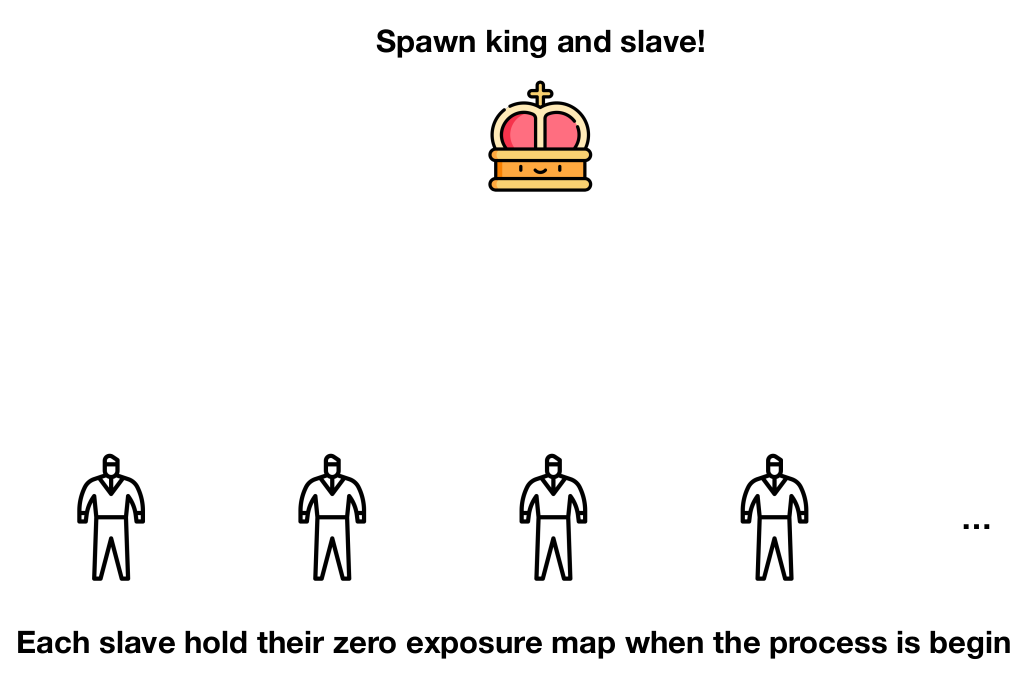
\includegraphics[width=0.7\textwidth]{content/methodology/figures/ms1}
    \caption{Spawning the king and slave processes}
    \label{fig:ms1}
\end{figure}

To begin with the calculation, initializing the exposure map with a 
separate workers and send multiple rows to the workers in the same amount
is trivial and waste a lot of resouces since there will be a fast worker 
who do a calculation really fast and the slow worker due to the cluster 
is composed of non-monolithic nodes with a different performance.
The trivial calculation will lock the resource in the cluster and blocks 
the other researcher who wants to run because the resouce allocation issue.
To maximize the usage of the CPU based cluster computing, there is a 
mechanism called ``Master-Slave technique''. The algorithm has been designed 
for utilizing the resource by spawning a king as the process manager 
and multiple slaves to be a process worker. The starting processs could 
be demonstrated in the Figure \ref{fig:ms1}. 


\begin{figure}[h!]
    \centering
    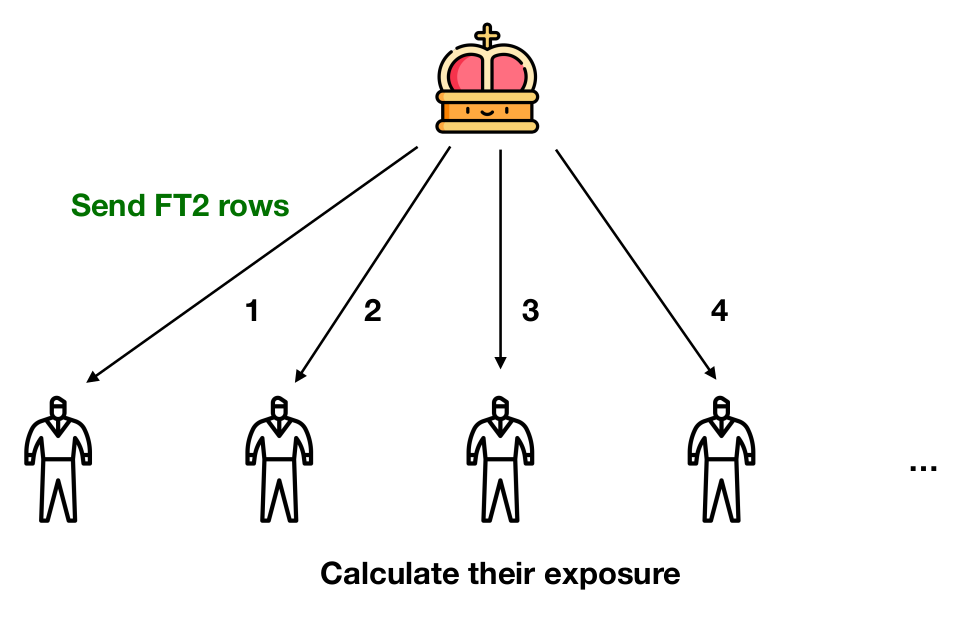
\includegraphics[width=0.7\textwidth]{content/methodology/figures/ms2}
    \caption{Master process send a small task to workers}
    \label{fig:ms2}
\end{figure}


\begin{figure}[h!]
    \centering
    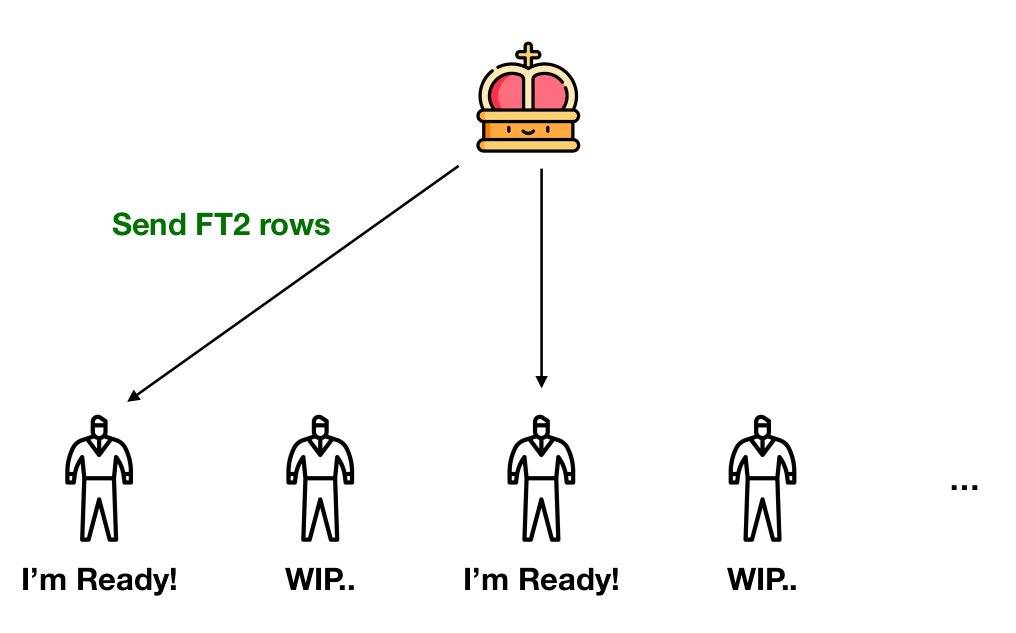
\includegraphics[width=0.7\textwidth]{content/methodology/figures/ms3}
    \caption{Aynchronous sending to an available worker}
    \label{fig:ms3}
\end{figure}


After that, the FT2 rows will be sent to slaves sequentially until
all workers hold a small chunk of data and do their jobs.
In practice, there is a metadata attach in the message. 
One of the option is the status tag. The status tag sends to the 
worker to declare the state of ther process whether it is in the 
calculation or the finishing. Figure \ref{fig:ms3} illustrates 
the non-sequential sending of the workload. The idea is simply 
sending a small task to an available worker and skip a busy worker
without disturbing them. This mechanism allows the exucution to utilize 
the resource in the cluster without wasting in the free worker.


By the end of the day, if the task is completely sent.
The master process will send the status tag as done to be an 
announcement of the finishing period. Then the exposure map of 
each worker will be gathered in the master process for superposition
and dump it to unify an exposure map. In addition, the calculation 
in an early period of testing is reported in Appendix \ref{appendix:exposure}.


\section{Hadronic Collision Model}
The proton spectrum power law in ridigity is described in Equation \ref{eq:spl}
as a single power law (SPL)
where the $\gamma$ represent the spectral index of the model. 
In fact, the spectrum has been observed as the differential flux 
in energy. Converting process between ridigity spectrum and the 
energy spectrum is derived in Appendix \ref{appendix:pw_energy} to 
obtain a precise calculation.


\textbf{Single power law (SPL)}
\begin{equation}
    \frac{dN}{dR} = R_0R^{-\gamma}
    \label{eq:spl}
\end{equation}

The most crucial part of this work is to determine if there is any 
breaking in the spectral indices in the power law. To represent 
a single breaking energy, broken power law (BPL) could be modeled 
the spectrum in ridigity as Equation \ref{eq:bpl}.


\textbf{Broken power law (BPL)}
\begin{equation}
\frac{dN}{dR}=
  \begin{cases}
    R_0R^{-\gamma_1}\ :\ E < E_{\text{Break}}\\
    R_0[R(E_{\text{Break}})]^{\gamma_2-\gamma_1}R^{-\gamma_2}\ :\ E \ge E_{\text{Break}}
  \end{cases}
  \label{eq:bpl}
\end{equation}

The scattering process of the hadronic collision from proton hitting 
the atmosphric molecules. The collision from incoming proton kinetic 
energy above 10 GeV could be modeled by proton-proton collision with 
an approximation that depends on the majority of the air components.
Model for the collision of proton-proton which yields $\gamma$-ray 
as a secondary product as a distribution in the spectrum has been 
derived in Equation \ref{eq:KO_model} from \cite{K&Omodel} work.

\begin{equation}
    \frac{dN_\gamma}{dE_\gamma} \propto \int^{E_{\text{max}}}_{E_\gamma} dE'\frac{dN_p}{dE'} \frac{d\sigma^{pp\rightarrow\gamma}(E',E_\gamma)}{dE_\gamma}
    \label{eq:KO_model}
\end{equation}

Where $d\sigma^{pp\rightarrow\gamma}(E',E_\gamma)/dE_\gamma$ contains 
a scattering amplitude of a given kinetic energy proton and the 
spectrum of the $\gamma$-ray. Atmosphric compoents mostly consists 
of nitrogen as the majority and the oxygon (\cite{atmosCompos}). The cross section from 
proton-proton collision and proton-nitrogen collision is roughly 
approximate as the multiplicative relation since there are plateau 
curve in the energy range in this analysis. The relation of the proton-proton 
scattering amplitude and the proton-nitrogen is obtained from \cite{WAtwater}
where it is highly depends on the atomic numbers of the air molecules. 

However, the second highest fraction of the arrival CR particles on 
Earth is an alpha ($\alpha$) particle. The helium nuclei can interact 
with the nitrogen and produces high energy $\gamma$-rays depends on
how much kinetic energy $\alpha$-particles is holding. Another 
estimation has been exploid by applying $\sigma_{\alpha N}/\sigma_{pN}$
to be a constant around 1.6 at the enegy range in GeV from 
the same relationship of proton-air collision model. Hence, derived
equation of the scattering process from incoming 
proton and $\alpha$-particle with air molecules to produce $\gamma$-ray
spectrum could be shown as Equation \ref{eq:derived_model}

\begin{equation}
    \frac{dN_{\gamma}}{dE_\gamma}(E_\gamma) \propto
    \sum_{E'_i}\left[\frac{E'_i}{E_{\gamma}}\Delta(\ln E'_i) \right]
    \left[ 
        f_{pp}\frac{dN_p}{dE'_i}
        \left\{
            1+\frac{\sigma_{\text{HeN}}}{\sigma{p\rm N}}\left(\frac{dN_p}{dR}\right)^{-1} \frac{dN_{\text{He}}}{dR} \frac{dR_{\text{He}}}{dR_p} 
        \right\}
    \right]
    ,\label{eq:derived_model}
\end{equation}

The CR helium spectrum would not be measured in this work 
since there will be a multiple parameters which leads to an overwhelming 
local optimum. The spectrum of $\alpha$-particles is directly measured 
by \cite{AMS-02Helium} and fix the distribution as one function rather 
modeled spectrum of CR proton spectrum. The full detail of the 
equation derivation will be demonstrated in \ref{appendix:interaction_model}.


% Eventhough converting process requires a derivation, the energy
% and ridigity of the proton particle could be approximate as the 
% same number for the lesser operation. Since the proton mass energy 
% is around 0.938 GeV/c$^2$. 

\section{Optimization}
Determining the best-fit spectral model requires an objectives function
to represent how well model match with an observed data. A proper 
methodology for fitting or optimization in another word is also 
a crucial part since there is likely that the local optimum exists 
in the parameters space. A poor optimization could lead the best-fit
stuck in a local minimum and yield a poor result. For better escaping 
local optima, heuristic optimization is employed for finding the 
best-fit of the model in parameter space.


\subsubsection{Poisson likelihood function}
An objective function is defined as Poisson likelihood function 
in the Equation \ref{eq:likelihood}. The reason behind the selection 
of Poisson function came from the observed model and measurement is 
considered as an amount of photons in each bin of the histogram. 
Converting the model spectrum to be a count histogram is simply 
multiplied by the integral of exposure map in limb region.

\begin{equation}
    \mathcal{L} = \prod_{i=1}^{N} P_{\text{pois}}(n_{\text{i,model}}, n_{\text{i,measurement}})
    \label{eq:likelihood}
\end{equation}

Since the spectrum order is in different order of magniture, then a
proper way to define an objective function is to redefine a
likelihood as a log-likelihood function for numerically
convenient like Eq \ref{eq:loglikelihood}. 

\begin{equation}
    Sum = \sum_{i=1}^{N} -\log P_{\text{pois}}(n_{\text{i,model}}, n_{\text{i,measurement}})
    \label{eq:loglikelihood}
\end{equation}

To sum up, a given proton spectrum yield a distrubution of $\gamma$-ray
spectrum to be converted into a count histogram and comparing with the 
real measurement. Not only for numerical convenient, but the negative sign 
also makes an algorithm to minimize the system rather than maximize 
a likelihood.

\subsubsection{Particle Swarm Optimization (PSO)}

The Early phase of the optimization, a plain gradient descent 
optimization has been used for model fitting. The result turns out 
that with a different initial parameters, the different best-fit model 
has changed which imply the local minimum in the problem. 
Even there is no method guarantee the global minimum but the heuristic
optimization could be a better option for handling this type of problem.
One kind of most widely used algorithm is particle swarm
optimization (PSO) and it is invented by \cite{pso_optimize}.

In order to get a best fit spectral indices, exploying the Particle Swarm Optimization (PSO)
by randomly initiate many particles in a given range of the parameter space and find the
local and global best fit in each step of iteration. Then rest of them would slowly moving
toward to the local and global position in parameter space with a proper weight. 
The iteration process will stop when the standard deviation of objective function from 
every particle less than a decimal. The explicit formula for every iteration $k$,
particle $i$ move with velocity $v_k^i$ is

\begin{equation}
    v^i_{k+1} = \omega v^i_k + c^br^b_k[b^i_k-x^i_k] + c^Br^B_k[B^i_k-x^i_k],
    \label{eq:pso}
\end{equation}
and updating the particle $i$ with
\begin{equation}
    x^i_{k+1} = x^i_k + v^i_{k+1}.
    \label{eq:pso_update}
\end{equation}
where
\begin{itemize}
    \item $x^i_k$ represent variable that particle $i$ hold
    \item $b$ and $B$ are best local and global parameter sets along the optimization process
    \item Set $\omega = 0.2$, $c^b = 0.2$ and $c^B = 0.3$
\end{itemize}

\section{Statistical significance}

Certainly, a larger model parameters or complexity would yield 
a better performance except it is overfitting the problem.
The critical issue is to answer how much significane the alternative 
model could outperform the trivial model. As the language of statistics 
would consider as two hypothesis. One for null and one for alternative 
approach. 

For this case, BPL has 2 more degree of freedom (DOF) than SPL.
Unquestionably, if there is a good optimization procedure, 
the objectives function would say BPL is better SPL. As mentioned 
from the previous paragraph, the significance level has to be taken
into account to put the weight on the study. Theoretically, regarding 
the model likelihood with a given set of parameters could be determined 
in the general case as Wilk's theorem define the realtion in 
Equation \ref{eq:wilk}.

\begin{equation}
    \mathcal{L} \equiv \prod_{\alpha=1}^n f(x_\alpha, \theta_1, \theta_2, ..., \theta_h)
    \label{eq:wilk}
\end{equation}
where 
\begin{itemize}
    \item $x_\alpha$ is represent a variant from model and data
    \item $\theta_i$ is a degree of freedom (DOF)
\end{itemize}

The practical usage to compare the null hypothesis and the alternative 
hypothesis as similar to one-tail hypothesis testing with a given 
dependency in more DOF has been adopted by \cite{Huelsenbeck}.
This method called ``Likelihood ratio test (LRT)''. The compact formula 
is shown in Equation \ref{eq:lrt}.

\begin{equation}
    \text{LRT} = -2\ln\left(\frac{\mathcal{L}_\text{null}}{\mathcal{L}_\text{alternative}}\right)
    \label{eq:lrt}
\end{equation}


\section{Error Determination}

Monte Carlo Simulation





